\newpage
\section{52. N皇后 II}
\label{leetcode:52}

\subsection{题目}

n 皇后问题研究的是如何将 n 个皇后放置在 n×n 的棋盘上,并且使皇后彼此之间不能相互攻击。

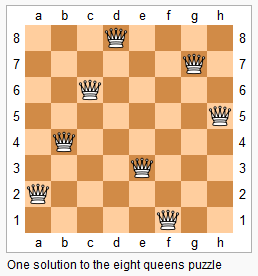
\includegraphics[width=50mm,height=50mm]{images/leetcode/8-queens.png}

上图为 8 皇后问题的一种解法。

给定一个整数 n,返回 n 皇后不同的解决方案的数量。

\textbf{示例}:

\begin{verbatim}
输入: 4
输出: 2
解释: 4 皇后问题存在如下两个不同的解法。
[
 [".Q..",  // 解法 1
  "...Q",
  "Q...",
  "..Q."],

 ["..Q.",  // 解法 2
  "Q...",
  "...Q",
  ".Q.."]
]
\end{verbatim}

\subsection{参考题解}

\begin{verbatim}
class Solution:
  def totalNQueens(self, n: int) -> int:
    self.count = 0
    def dfs(cols, pie, na, row):
      if row >= n:
        self.count += 1
        return
      for col in range(n):
        if (col not in cols) and (row + col not in pie) and (row - col not in na):
          dfs(cols|{col}, pie|{row+col}, na|{row-col}, row+1)
    dfs(set(), set(), set(), 0)
    return self.count
\end{verbatim}

\subsection{参考题解,位运算}

列,撇,捺 这 3 个 set 可以用位运算来优化,只需要用一个整数即可。

\begin{verbatim}
class Solution:
  def totalNQueens(self, n: int) -> int:
    self.count = 0
    def dfs(cols, pie, na, row):
      if row >= n:
        self.count += 1
        return
      bits = (~(cols|pie|na)) & ((1<<n) - 1) # 得到当前所有的空位
      while bits:
        p = bits & -bits # 取到最低位的1
        bits = bits & (bits - 1) # 表示在p位置上放入皇后
        dfs(cols|p, (pie|p)<<1, (na|p)>>1, row+1)
    dfs(0, 0, 0, 0)
    return self.count
\end{verbatim}
